\documentclass{article}
\usepackage{microtype}
\usepackage[utf8]{inputenc} 
\usepackage[a4paper, total={6in, 9.6in}]{geometry}
\usepackage{enumitem}
\usepackage{amsmath}
\usepackage{amssymb}
\usepackage{fancyhdr}
\usepackage{xcolor}
\usepackage{tikz}
\usepackage{pgfplots}
\usepackage{svg}
\usepackage{graphicx}
\usepackage{listings}

\widowpenalties=4 10000 10000 150 0


% listings sonderzeichen
\lstset{
  literate={ö}{{\"o}}1
           {ä}{{\"a}}1
           {ü}{{\"u}}1
}
\lstdefinelanguage
   [x64]{Assembler}     % add a "x64" dialect of Assembler
   [x86masm]{Assembler} % based on the "x86masm" dialect
   % with these extra keywords:
   {morekeywords={CDQE,CQO,CMPSQ,CMPXCHG16B,JRCXZ,LODSQ,MOVSXD, %
                  POPFQ,PUSHFQ,SCASQ,STOSQ,IRETQ,RDTSCP,SWAPGS, %
                  rax,rdx,rcx,rbx,rsi,rdi,rsp,rbp, %
                  r8,r8d,r8w,r8b,r9,r9d,r9w,r9b, %
                  r10,r10d,r10w,r10b,r11,r11d,r11w,r11b, %
                  r12,r12d,r12w,r12b,r13,r13d,r13w,r13b, %
                  r14,r14d,r14w,r14b,r15,r15d,r15w,r15b}} % etc.

% header / footer style
\pagestyle{fancy}
\fancyhf{}
\rhead{Systemnahe Informatik SS20}
\lhead{Stefan Schmauch, Anton Lydike}
\rfoot{Seite \thepage}

% define some basic colors
\definecolor{greeen}{RGB}{34,139,34}
\newcommand\red[1]{\textcolor{red}{#1}}
\newcommand\green[1]{\textcolor{greeen}{#1}}
\newcommand\blue[1]{\textcolor{blue}{#1}}


% define a task 
\newcommand\task[2]{\noindent\textbf{Aufgabe #1)\hfill \underline{\,\,\,\,\,\,}\,\,/#2p.}\\}
% and the total points for this sheet
\newcommand\pointsttl[1]{\noindent\textbf{Gesamtpunkte: \hfill \underline{\,\,\,\,\,\,}\,\,/#1p.}\\}


\newcommand\cfgtitle[1]{\title{\vspace{-1.5cm}Übungsblatt #1\\%
\begin{large} Übungsgruppe Pentium \end{large}} \lfoot{Übungsblatt #1}\cfoot{Übungsgruppe Pentium}}
\author{Stefan Schmauch, Anton Lydike}


\usepackage{tikz}
\usetikzlibrary{arrows,automata}   

\cfgtitle{3}
\date{Donnerstag 14.05.2020}

\begin{document}
    \maketitle
    \thispagestyle{fancy}

    \task{1}{5}

    \lstinputlisting{1.asm}

    \task{2}{4}

    \lstinputlisting{2.asm}

    \task{3}{6}
    \lstinputlisting{3.asm}
    
    \task{4}{2+3+3}
    \begin{enumerate}[label=\alph*)]
        \item \hfill \begin{center}
            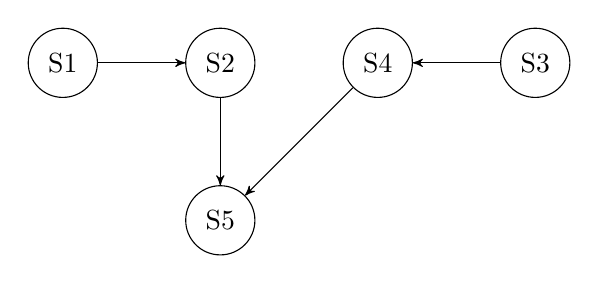
\begin{tikzpicture}[->,>=stealth',node distance=2cm]
                \node[state] (S1) {S1};
                \node[state] (S2) [right of=S1]  {S2};
                \node[state] (S5) [below of=S2] {S5};
                \node[state] (S4) [right of=S2] {S4};
                \node[state] (S3) [right of=S4] {S3};
    
                \path (S1) edge (S2)
                      (S2) edge (S5)
                      (S3) edge (S4)
                      (S4) edge (S5);
            \end{tikzpicture}
        \end{center}

        \item \hfill
        \lstinputlisting{4b.asm}
        \item \hfill
        \lstinputlisting{4c.asm}
    \end{enumerate}

    \pointsttl{23}
\end{document}

